\documentclass{article}[12 pt]
\usepackage{amssymb}
\usepackage{amsthm}
\usepackage{amsmath}
\usepackage{appendix}
\usepackage{array}
\usepackage{geometry}
\usepackage{enumitem}
\usepackage{graphicx}
\usepackage{subfig}
\usepackage{caption}
\usepackage{url}
\usepackage{float}
\usepackage{pdfpages}
\usepackage{shortvrb}
\usepackage{mathtools}
\usepackage{multirow}
\usepackage{hyperref}
\usepackage{commath}
\usepackage{bm}


\def\BibTeX{{\rm B\kern-.05em{\sc i\kern-.025em b}\kern-.08em
		T\kern-.1667em\lower.7ex\hbox{E}\kern-.125emX}}


\graphicspath{{"/media/edrive/Bayesian_Methods/BHM_Assignments/HW02/Report/Images/"}}
\geometry{margin=1 in}

\newcommand{\smallvskip}{\vspace{5 pt}}
\newcommand{\medvskip}{\vspace{30 pt}}
\newcommand{\bigvskip}{\vspace{100 pt}}
\newcommand{\tR}{\mathtt{R}}




\begin{document}
	
\begin{center}
	\textbf{\Large Connor McCurley} \\
	AGR 6932  \qquad \quad \quad \textbf{\large Homework 2} \quad \quad \qquad Fall 2019 
\end{center}


%===================================================
%=================== Question 1 ====================
%===================================================

\section*{Question 1}
A \textit{probability mass function} operates on discrete random variables.  Its evaluation returns the probability that a random variable will take on the value of its argument.  A \textit{probability  density function}, on the other hand, operates over continuous random variables.  Probability density functions do not return probability values, but probability densities. Integration must be applied to return the probability over an interval. \\

\noindent
As stated in the class textbook, a \textit{random variable} is a quantity that can take on values due to chance.  They do not have a single value, but instead can take on a range of values.  The important distinction between random variables and the parameters of a probability distribution is that random variables are governed by probability distributions (and hence the parameters of the distributions).  In some cases, the parameters of a distribution can also be modeled as a random variables. 


%===================================================
%=================== Question 2 ====================
%===================================================
\section*{Question 2}
The following plots demonstrate convergence of the Binomial and Poisson distributions to a Normal.

\begin{figure}[H]%
	\centering
	\subfloat[Nose]{{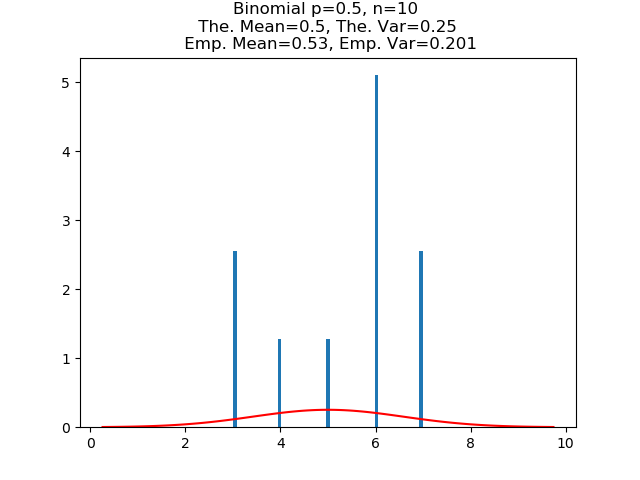
\includegraphics[width=5cm]{q2_bin_10} }}%
	\qquad
	\subfloat[Mouth]{{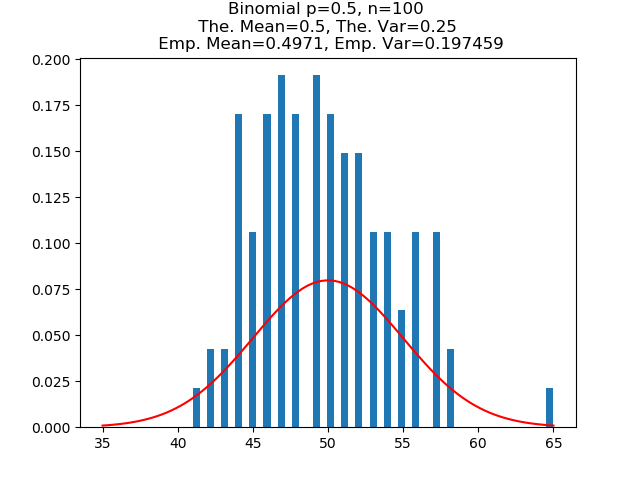
\includegraphics[width=5cm]{q2_bin_100} }}%
	\qquad
	\subfloat[Left Eye]{{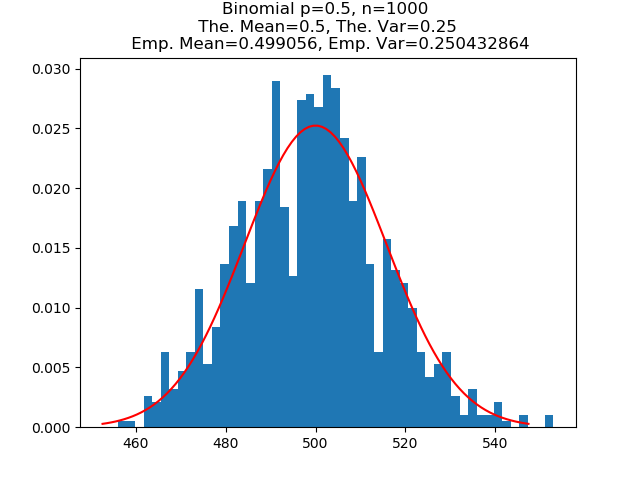
\includegraphics[width=5cm]{q2_bin_1000} }}%
	\qquad
	\subfloat[Right Eye]{{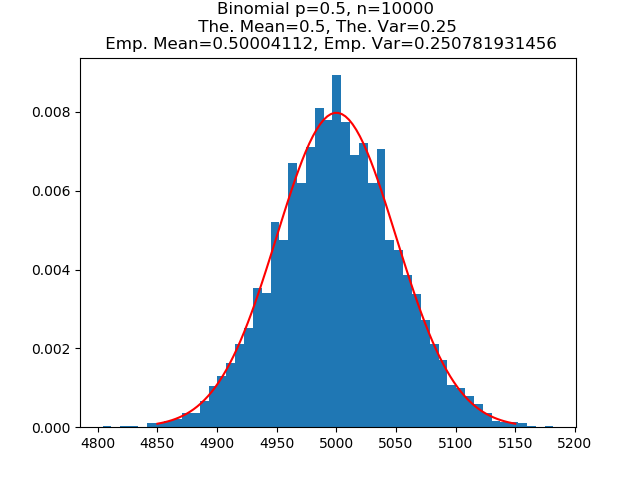
\includegraphics[width=5cm]{q2_bin_10000} }}%
	\qquad
	\subfloat[Left Eye]{{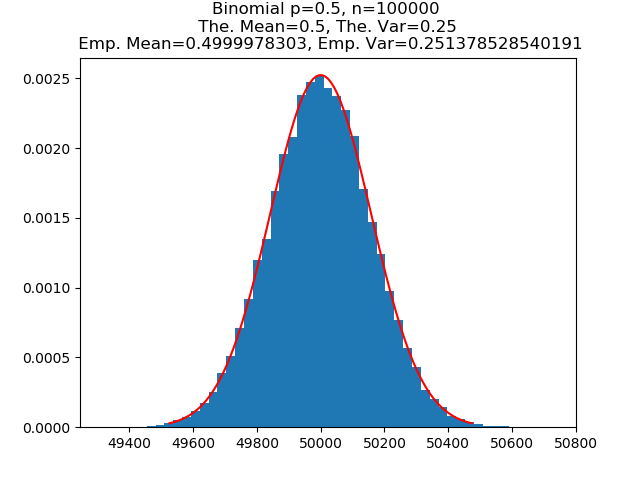
\includegraphics[width=5cm]{q2_bin_100000} }}%
	\qquad
	\subfloat[Right Eye]{{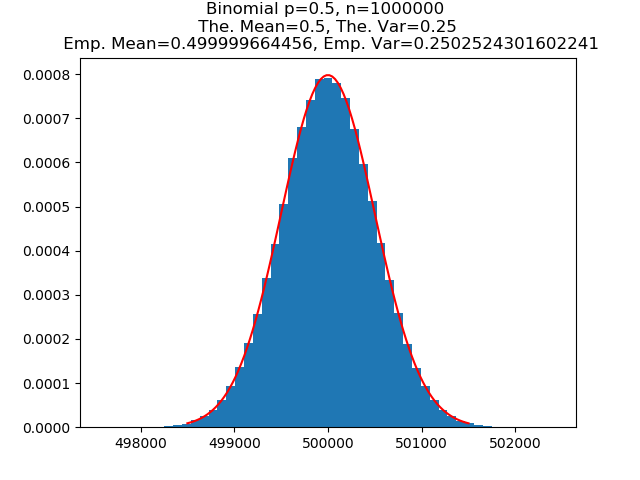
\includegraphics[width=5cm]{q2_bin_1000000} }}%
	\caption{}%
	\label{fig:q2_bin_to_normal}%
\end{figure}

\begin{figure}[H]%
	\centering
	\subfloat[Nose]{{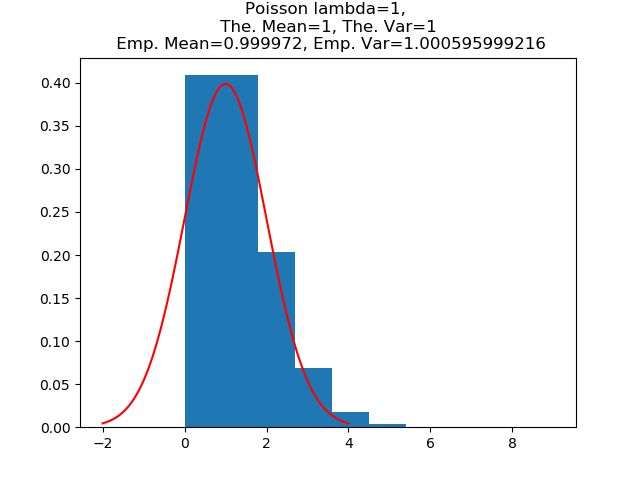
\includegraphics[width=5cm]{q2_pois_1} }}%
	\qquad
	\subfloat[Mouth]{{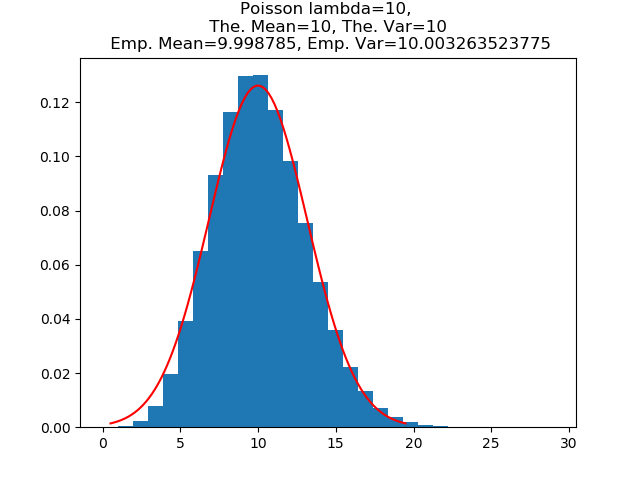
\includegraphics[width=5cm]{q2_pois_10} }}%
	\qquad
	\subfloat[Left Eye]{{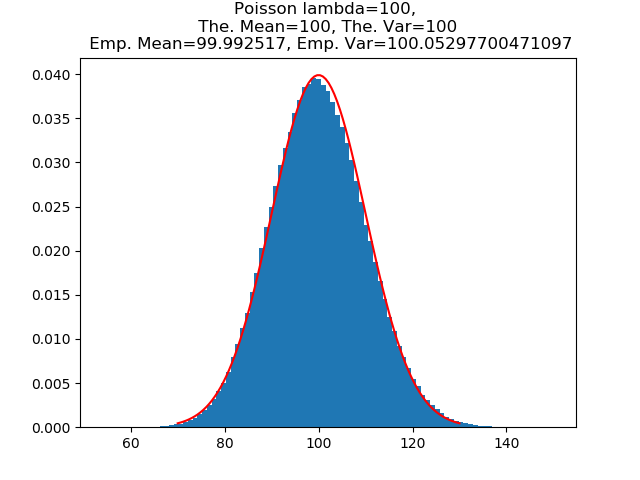
\includegraphics[width=5cm]{q2_pois_100} }}%
	\qquad
	\subfloat[Right Eye]{{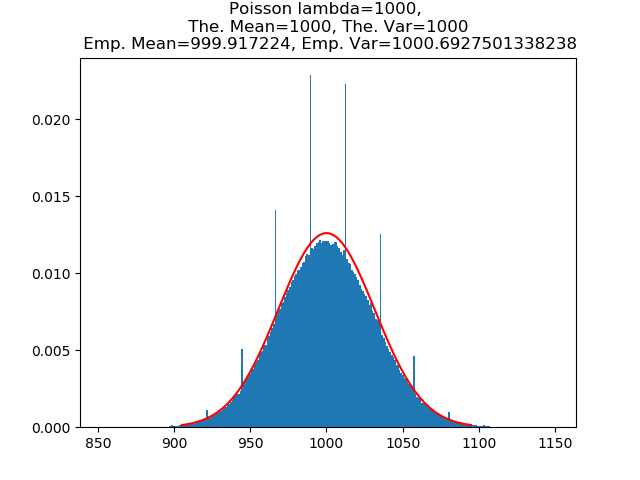
\includegraphics[width=5cm]{q2_pois_1000} }}%
	\caption{}%
	\label{fig:q2_pois_to_normal}%
\end{figure}

%===================================================
%=================== Question 3 ====================
%===================================================
\section*{Question 3}

\begin{center}
	\begin{figure}[h]
		\centering
		\includegraphics[width=0.75\textwidth]{"q3_gamma_skew"}
		\caption{ }
		\label{fig:q3_gamma_skew}
	\end{figure}
\end{center}


%===================================================
%=================== Question 4 ====================
%===================================================
\section*{Question 4}


%===================================================
%=================== Question 5 ====================
%===================================================
\section*{Question 5}

\begin{figure}[H]%
	\centering
	\subfloat[Nose]{{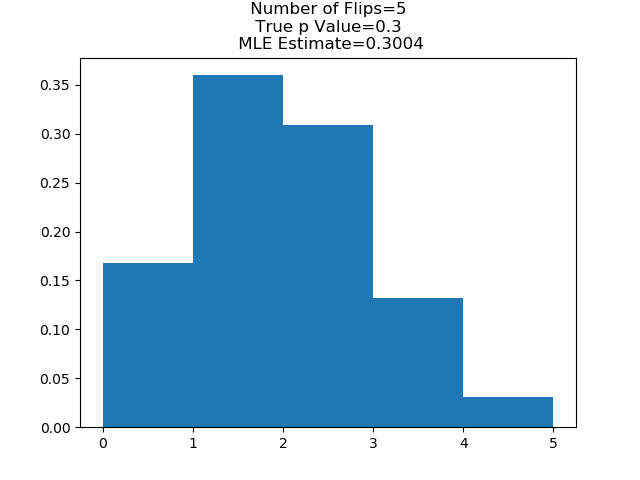
\includegraphics[width=5cm]{q5_mle_5} }}%
	\qquad
	\subfloat[Mouth]{{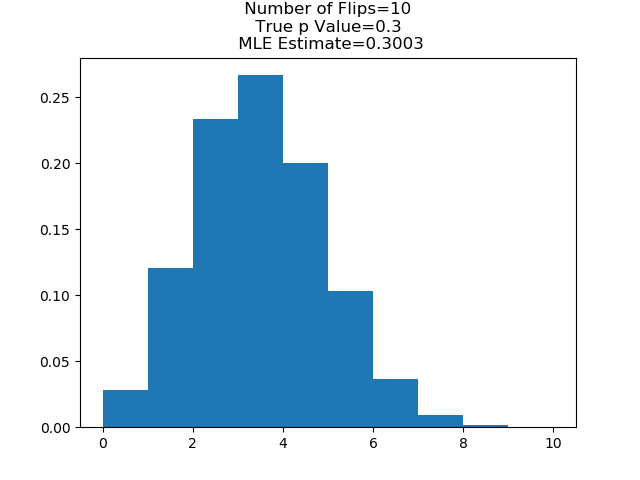
\includegraphics[width=5cm]{q5_mle_10} }}%
	\qquad
	\subfloat[Left Eye]{{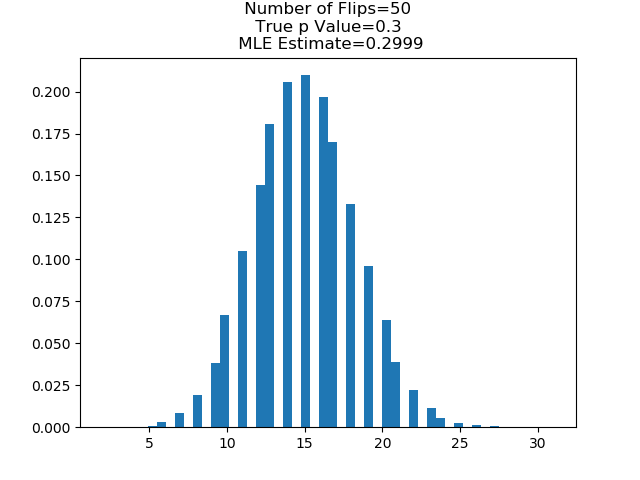
\includegraphics[width=5cm]{q5_mle_50} }}%
	\qquad
	\subfloat[Right Eye]{{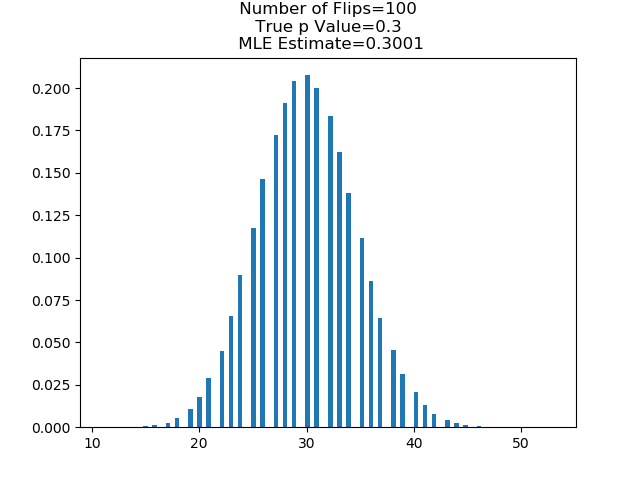
\includegraphics[width=5cm]{q5_mle_100} }}%
	\caption{}%
	\label{fig:q5_mle}%
\end{figure}

\begin{figure}[H]%
	\centering
	\subfloat[Nose]{{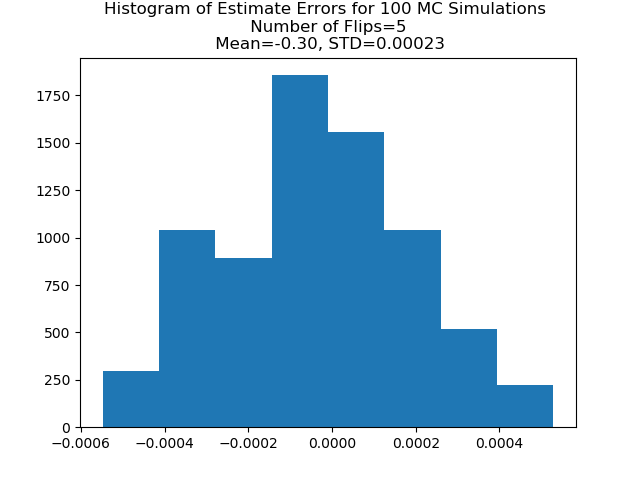
\includegraphics[width=5cm]{q5_mc_5} }}%
	\qquad
	\subfloat[Mouth]{{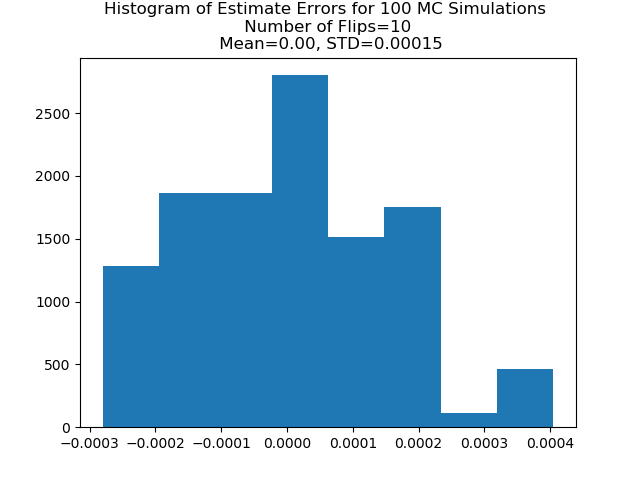
\includegraphics[width=5cm]{q5_mc_10} }}%
	\qquad
	\subfloat[Left Eye]{{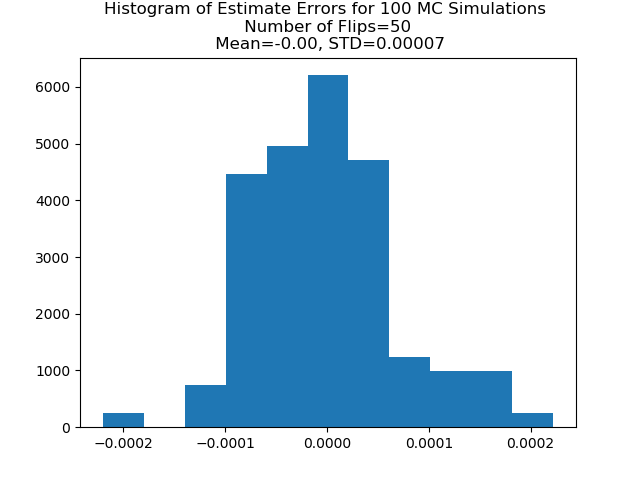
\includegraphics[width=5cm]{q5_mc_50} }}%
	\qquad
	\subfloat[Right Eye]{{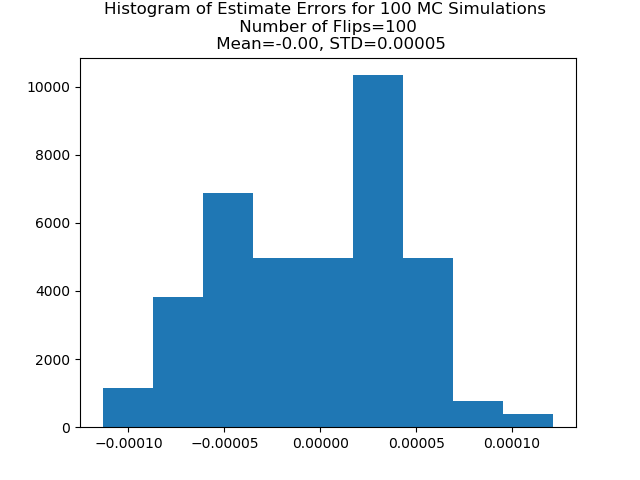
\includegraphics[width=5cm]{q5_mc_100} }}%
	\caption{}%
	\label{fig:q5_mc}%
\end{figure}


%===================================================
%=================== Question 6 ====================
%===================================================
\section*{Question 6}

\begin{center}
	\begin{figure}[h]
		\centering
		\includegraphics[width=0.75\textwidth]{"q6_trajectories"}
		\caption{ }
		\label{fig:q6_trajectories}
	\end{figure}
\end{center}

\begin{center}
	\begin{figure}[h]
		\centering
		\includegraphics[width=0.75\textwidth]{"q6_observation_error"}
		\caption{ }
		\label{fig:q6_observation_error}
	\end{figure}
\end{center}

\begin{center}
	\begin{figure}[h]
		\centering
		\includegraphics[width=0.75\textwidth]{"q6_process_error"}
		\caption{ }
		\label{fig:q6_process_error}
	\end{figure}
\end{center}


\end{document}
